%
% galois.tex -- Abschnitt über Galois-Körper
%
% (c) 2020 Prof Dr Andreas Müller, Hochschule Rapperswil
%
% !TeX spellcheck = de_CH
\section{Galois-Körper
\label{buch:section:galoiskoerper}}
\rhead{Galois-Körper}
Ein Körper $\Bbbk$ enthält mindestens die Zahlen $0$ und $1$.
Die Null ist nötig, damit $\Bbbk$ eine Gruppe bezüglich der
Addition ist, die immer ein neutrales Element, geschrieben $0$,
enthält.
Die Eins ist nötig, damit $\Bbbk^*=\Bbbk\setminus\{0\}$ eine
Gruppe bezüglich der Multiplikation ist, die immer eine neutrales
Element, geschrieben $1$, enthält.
Durch wiederholte Addition entstehen auch die Zahlen $2=1+1$, $3=2+1$ 
und so weiter.
Es sieht also so aus, als ob ein Körper immer unendliche viele
Elemente enthalten müsste.
Wie können also endliche Körper entstehen?

In diesem Abschnitt sollen die sogenannten Galois-Körper $\mathbb{F}_p$
\index{Galois-Körper}%
\index{Fp@$\mathbb{F}_p$}%
mit genau $p$ Elementen konstruiert werden, die es für jede Primzahl $p$ gibt.
Sie sind die Basis für weitere endliche Körper, die eine beliebige
Primzahlpotenz $p^n$ von Elementen haben und die die Basis wichtiger
kryptographischer Algorithmen sind.

%
% Arithmetik modulo $o$
%
\subsection{Arithmetik modulo $p$
\label{buch:subsection:arithmetik-modulo-p}}
Damit aus den Zahlen $0, 1, 2, \dots$ ein endlicher Körper werden kann,
muss die Folge sich wiederholen.
Schreiben wir $a_0=0,a_1=1,\dots$ für die Folge, dann muss es also
ein Folgenelement $a_k$ geben und ein $n$ derart, dass $a_{k+n}=a_{k}$.
Dies bedeutet, dass $k+n = k$ sein muss.
Subtrahiert man $k$ auf beiden Seiten, dann folgt, dass $n=0$ sein muss.
Damit ein endlicher Körper entsteht, muss also die Menge
\begin{align*}
&\{0,1,2,\dots,n-1\}
\intertext{eine Gruppe bezüglich der Addition sein, und}
&\{1,2,\dots,n-1\}
\end{align*}
eine Gruppe bezüglich der Multiplikation.

\subsubsection{Restklassenring}
Wir definieren die Grundoperationen in einer Menge, die mit den
Zahlen $\{0,1,2,\dots,n-1\}$ identifiziert werden kann.

\begin{definition}
Die Zahlen $a,b\in\mathbb{Z}$ heissen {\em kongruent modulo $n$},
\index{kongruent modulo $n$}%
geschrieben
\[
a\equiv b\mod n,
\]
wenn $a-b$ durch $n$ teilbar ist, also $n|(a-b)$.
\end{definition}

Die Zahlen mit gleichem Rest sind Äquivalenzklassen der Kongruenz modulo $n$.
Die Zahlen mit Rest $k$ modulo $n$ bilden die {\em Restklasse}
\index{Restklasse}%
\[
\llbracket k\rrbracket=\{\dots,k-2n,k-n,k,k+n,k+2n,\dots\} \subset\mathbb{Z}.
\]
Sie bilden eine endliche Menge, die man mit den Resten $0,1,\dots,n-1$
identifizieren kann.

\begin{definition}
Die Menge $\mathbb{Z}/n\mathbb{Z}$ besteht aus den Restklassen
$\llbracket 0\rrbracket,\llbracket 1\rrbracket,\dots,\llbracket n-1\rrbracket$,
die auch einfach $0,1,\dots,n-1$ geschrieben werden.
\end{definition}

Beim Rechnen mit Resten modulo $n$ können Vielfache von $n$ ignoriert werden.
Zum Beispiel gilt 
\[
\begin{aligned}
48&\equiv -1\mod 7&&\Leftrightarrow& 48&=-1&&\text{in $\mathbb{Z}/7\mathbb{Z}$}
\\
3\cdot 5=15&\equiv\phantom{-}1\mod 7&&\Leftrightarrow & 3\cdot 5&=\phantom{-}1&&\text{in $\mathbb{Z}/7\mathbb{Z}$.}
\end{aligned}
\]
Das Beispiel zeigt, dass man mindestens in $\mathbb{Z}/7\mathbb{Z}$ mit
Resten ganz ähnlich rechnen kann wie in $\mathbb{Q}$.
In $\mathbb{Z}/7\mathbb{Z}$ scheinen $3$ und $5$ multiplikative Inverse
zu sein.

Tatsächlich kann man auf den Restklassen eine Ringstruktur definieren.
Dazu muss man sicherstellen, dass die Auswahl eines Repräsentanten keinen
Einfluss auf den Rest hat.
Der Rest $a$ kann jede Zahl der Form $a+kn$ darstellen.
Ebenso kann der Rest $b$ jede Zahl der Form $b+ln$ darstellen.
Deren Summe ist $a+b+(k+l)n\equiv a+b\mod n$.
Der Repräsentant des Restes hat also keinen Einfluss auf die Summe.
Ebenso ist das Produkt der beiden Repräsentaten 
$(a+kn)\cdot(b+ln) = ab + (al+bk)n + kln^2=ab + (al+bk+kln)n\equiv ab\mod n$
für jede Wahl von $k$ und $l$.
Auch die Multiplikation ist also unabhängig vom gewählten Repräsentanten.

\begin{definition}
Die Menge $\mathbb{Z}/n\mathbb{Z}$ ist ein Ring,
er heisst der {\em Restklassenring modulo $n$}.
\end{definition}

\subsubsection{Division in $\mathbb{Z}/n\mathbb{Z}$}
Um einen endlichen Körper zu erhalten, muss die Menge
\[
\mathbb{Z}/n\mathbb{Z} \setminus \{\llbracket0\rrbracket\}
=
\{
\llbracket 1\rrbracket,
\llbracket 2\rrbracket,
\dots
\llbracket n-q\rrbracket
\}
\]
eine Gruppe bezüglich der Multiplikation sein.
Insbesondere darf kein Produkt $a\cdot b$ mit Faktoren in 
$\mathbb{Z}/n\mathbb{Z} \setminus \{\llbracket0\rrbracket\}$
zu Null werden.
Für $n=15$ funktioniert dies nicht, das Produkt $3\cdot 5\equiv 0\mod 15$.
Wir kommen daher zu der Forderung, dass der Ring $\mathbb{Z}/n\mathbb{Z}$ 
nur dann ein Körper sein kann, wenn er nullteilerfrei ist.

Falls sich $n=p_1\cdot p_2$ in zwei Faktoren zerlegen lässt, dann sind
$p_1$ und $p_2$ Nullteiler in $\mathbb{Z}/n\mathbb{Z}$.
Ein Körper kann also nur entstehen, wenn $n$ eine Primzahl ist.

\begin{definition}
\label{buch:endlichekoerper:def:galois-koerper}
Ist $p$ eine Primzahl, dann heisst $\mathbb{F}_p=\mathbb{Z}/p\mathbb{Z}$
\index{Primzahl}%
der Galois-Körper der Ordnung $p$.
\index{Galois-Körper}%
\end{definition}

Diese Definition ist nur gerechtfertigt, wenn $\mathbb{F}_p^*$ tatsächlich
eine Gruppe ist, wenn also jede Zahl zwischen $1$ und $p-1$ ein Inverses
bezüglich der Multiplikation hat.
Zu einem Rest $a\in\mathbb{F}_p^*$ muss also ein Rest $b$ gefunden werden,
so dass $ab\equiv 1\mod p$.
Dies ist gleichbedeutend mit Zahlen $b$ und $n$ derart, dass
\begin{equation}
ab+np=1.
\label{buch:endliche-koerper:teilerfremd}
\end{equation}
In~\eqref{buch:endliche-koerper:teilerfremd} sind $a$ und $p$ gegeben,
gesucht sind $b$ und $n$.

In Abschnitt~\ref{buch:section:euklid} wurde gezeigt, wie der euklidische
Algorithmus eine Gleichung der Form~\eqref{buch:endliche-koerper:teilerfremd}
lösen kann, wenn die beiden gegebenen Zahlen $a$ und $p$ teilerfremd sind.
Dies ist aber dadurch garantiert, dass $p$ eine Primzahl ist und $1\le a <p$.
Die multiplikative Inverse von $a$ in $\mathbb{F}_p^*$ kann also mit
Hilfe des euklidischen Algorithmus effizient gefunden werden.
\index{multiplikative Inverse in $\mathbb{F}_p$}%

\begin{beispiel}
Die kleinste Primzahl grösser als $2021$ ist $p=2063$.
Was ist die Inverse von $2021$ in $\mathbb{F}_{2063}$?

Wir führen den euklidischen Algorithmus für das Paar $(2063,2021)$ durch
und erhalten 
\begin{center}
\begin{tabular}{|>{$}c<{$}|>{$}r<{$}|>{$}r<{$}|>{$}r<{$}|>{$}r<{$}|}
\hline
k&  a_k&  b_k& q_k& r_k\\
\hline
0& 2063& 2021&   1&  42\\
1& 2021&   42&  48&   5\\
2&   42&    5&   8&   2\\
3&    5&    2&   2&   1\\
4&    2&    1&   2&   0\\
\hline
\end{tabular}
\end{center}
Die gesuchten Faktoren $b$ und $n$ können aus dem Matrizenprodukt
$Q(q_n)\dots Q(q_0)$ gefunden werden:
\begin{align*}
Q
&=
\begin{pmatrix} 0& 1\\ 1& -2 \end{pmatrix}
\begin{pmatrix} 0& 1\\ 1& -2 \end{pmatrix}
\begin{pmatrix} 0& 1\\ 1& -8 \end{pmatrix}
\begin{pmatrix} 0& 1\\ 1& -48 \end{pmatrix}
\begin{pmatrix} 0& 1\\ 1& -1 \end{pmatrix}
\\
&=
\begin{pmatrix} 0& 1\\ 1& -2 \end{pmatrix}
\begin{pmatrix} 0& 1\\ 1& -2 \end{pmatrix}
\begin{pmatrix} 0& 1\\ 1& -8 \end{pmatrix}
\begin{pmatrix} 1& -1\\ -48& 49\end{pmatrix}
\\
&=
\begin{pmatrix} 0& 1\\ 1& -2 \end{pmatrix}
\begin{pmatrix} 0& 1\\ 1& -2 \end{pmatrix}
\begin{pmatrix} -48& 49\\ 385& -393 \end{pmatrix}
\\
&=
\begin{pmatrix} 0& 1\\ 1& -2 \end{pmatrix}
\begin{pmatrix} 385& -393\\ -818& 835 \end{pmatrix}
\\
&=
\begin{pmatrix} -818&   835\\ 2021& -2063\end{pmatrix}.
\end{align*}
Daraus können wir ablesen, dass
\[
-818\cdot 2021 +835 \cdot 2063=1.
\]
Der Rest $ -818\equiv 1245\mod 2063$ ist also die multiplikative
Inverse von $2021$ in $\mathbb{F}_{2063}$.
\end{beispiel}

\subsubsection{Der kleine Satz von Fermat}
\index{Fermat, kleiner Satz von}%
\index{kleiner Satz von Fermat}%
In $\mathbb{Z}$ wachsen die Potenzen einer Zahl immer weiter an.
In einem endlichen Körper kann dies nicht gelten, da nur endlich
viele Werte zur Verfügung stehen.
Tatsächlich müssen die Potenzen einer von $0$ verschiedenen Zahl
$a\in\mathbb{F}_p^*$ alle in $\mathbb{F}_p^*$ liegen.
Es gibt aber nur $p-1$ Zahlen in $\mathbb{F}_p^*$, spätestens
die Potenz mit Exponent $p$ muss also mit einer früheren Potenz
übereinstimmen.
Der kleine Satz von Fermat sagt etwas genauer: die $p$-te Potenz
von $a$ ist genau die Zahl $a$:

\begin{figure}
\centering
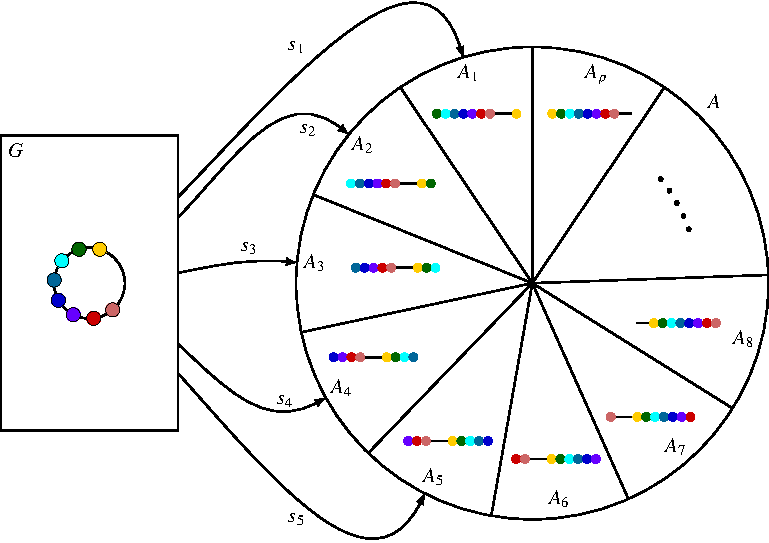
\includegraphics{chapters/30-endlichekoerper/images/fermat.pdf}
\caption{$G$ ist die Menge aller verschiedenfarbigen geschlossenen
Perlenketten mit $p$ Perlen und $a$ Farben.
$A$ ist die Menge aller linearen verschiedenfarbigen Ketten.
Die Abbildung $s_i$ schneidet die Ketten an der Stelle $i$ auf,
dadurch entstehen die Menge $A_i$, verschiedenfarbigen linearen
Ketten der Länge $p$ mit $a$ Farben.
Die Abbildungen $s_i$ sind injektiv, die Mengen $A_i$ haben alle
die gleiche Anzahl Elemente.
Genau dann ist $|A|$ durch $p$ teilbar, wenn die Mengen $A_i$
disjunkt sind.
\label{buch:endliche-koerper:fig:fermat}}
\end{figure}

\begin{satz}[Kleiner Satz von Fermat]
\label{buch:endliche-koerper:satz:fermat}
In $\mathbb{F}_p$ gilt $a^p=a$ für alle $a\in\mathbb{F}_p^*$.
\end{satz}

Wir beweisen diesen Satz in der folgenden, traditionelleren 
Formulierung.

\begin{satz}
Für jede ganze Zahl $a>0$ gilt $p|(a^p-a)$ genau dann, wenn
$p$ eine Primzahl ist.
\end{satz}

\begin{proof}[Beweis]
Wir müssen zeigen, dass $p$ ein Teiler ist von $a^p-a$.
Das nachfolgende kombinatorische Argument wird zum Beispiel
von Mathologer auf seinem Youtube-Kanal im Video
\url{https://youtu.be/_9fbBSxhkuA} illustriert.

Zum Beweis interpretieren wir die vorkommenden Zahlen kombinatorisch.
Die Zahl $a^p$ ist die Anzahl der verschiedenen Perlenketten der Länge
$p$, die sich aus Glasperlen mit $a$ verschiedenen Farben herstellen
lassen.
Davon bestehen $a$ Perlenketten aus nur einer einzigen Farbe.
Die Zahl $a^p-a$ ist also die Anzahl der Perlenketten der Länge $p$
aus Glasperlen mit $a$ verschiedenen Farben, die mindestens zwei
verschiedene Farben verwenden.
Wir bezeichnen die Menge der nicht einfarbigen Perlenketten der
Länge $p$ mit $a$ Farben mit $A$.
Es ist $|A|=a^p-a$.

Zu sagen, dass $a^p-a$ durch $p$ teilbar ist, ist gleichbedeutend
damit, dass die Menge der Perlenkette in $p$
disjunkte, gleichmächtige Mengen aufgeteilt werden kann.
Es ist also zu zeigen, dass sich die Menge $A$ genau dann in
disjunkte gleichmächtige Mengen zerlegen lässt, wenn $p$ eine
Primzahl ist.

Wir betrachten dazu die Menge der nicht einfarbigen, geschlossenen
Perlenketten der Länge $p$ mit $a$ Farben.
Einge dieser Perlenketten unterscheiden sich nur durch eine
Drehung um eine gewisse Anzahl Perlen.
Sei $G$ die Menge der nicht einfarbigen, geschlossenen
Perlenketten, die sich nicht nur um eine Drehung unterscheiden.

Die Abbildung $s_i\colon G\to A$
in Abbildung~\ref{buch:endliche-koerper:satz:fermat} 
schneidet die Perlenkette in $G$ an der Stelle $i$ auf.
Diese Abbildungen sind ganz offensichtlich injektiv.
Die Bildmengen $A_i = s_i(G)$ haben daher alle gleich
viele Elemente wie $G$: $|A_i|=|G|$.

Da jede lineare Perlenkette in $A$ durch geeignetes Aufschneiden
einer geschlossenen Perlenkette in $G$ entsteht, ist 
\[
A=\bigcup_{i=1}^p A_i.
\]

Wir müssen jetzt nur noch untersuchen, unter welchen Bedingungen
die Mengen $A_i$ disjunkt sind.
Zwei Mengen $A_i$ und $A_j$ enthalten genau dann eine
gemeinsame Perlenkette, wenn es eine geschlossene Kette in $G$
gibt, die beim Aufschneiden an den Stellen $i$ und $j$ die
gleiche Kette ergeben.
Dies bedeutet, dass sich die Farben zwischen $i$ und $j$ nach
der Stelle $j$ wiederholen.
Die Mengen sind also genau dann nicht disjunkt, wenn es
peridische Ketten gibt mit einer Periode $k<p$.

Da die Periode einer periodischen Kette ein Teiler von $p$
ist, gibt es genau dann keine periodischen Ketten, wenn $p$
eine Primzahl ist.
Damit ist die Behauptung gezeigt.
\end{proof}

Der kleine Satz von Fermat kann auch dazu verwendet werden, Potenzen 
in $\mathbb{F}_p$ zu vereinfachen, wie das folgende Beispiel\footnote{%
Das Beispiel stammt aus dem Video~\url{https://youtu.be/_9fbBSxhkuA},
welches Mathologer zu Halloween 2018 veröffentlich hat}
zeigt.

\begin{beispiel}
Man berechnet in $\mathbb{F}_{13}$ die Potenz $11^{666}$.
Nach dem kleinen Satz von Fermat ist $11^{13} = 11$ oder $11^{12}=1$,
man kann also den Exponenten modulo $12$ reduzieren.
Weil $666=55\cdot 12 + 6$ erhält man $11^{666}= 11^6$.
Da die Potenzen von $11$ etwas mühsam zu berechnen sind,
kann man sie wegen $11=-2$ in $\mathbb{F}_{13}$ auch als Potenzen
von $-2$ bekommen.
Aber $(-2)^6 = 64 = -1 \in\mathbb{F}_{13}$.
\end{beispiel}

In der Form $a^{p-1}=1$ in $\mathbb{F}_p$ liefert der kleine Satz
von Fermat die Inverse von $a$ als $a^{p-2}$.
Dies bedeutet zum Beispiel, dass in $\mathbb{F}_3$ jede von $0$
verschiedene Zahl zu sich selbst invers ist: $1\cdot 1=1$ und $2\cdot 2=1$.
Diese Art, die Inverse zu bestimmen, ist allerdings nicht effizienter
als der euklidische Algorithmus, aber sie ist manchmal für
theoretische Überlegungen nützlich.

\subsubsection{Der Satz von Wilson}
Der Satz von Wilson ermöglicht, die multiplikative Inverse auf eine
andere Art zu berechnen.
Sie ist zwar nicht unbedingt einfacher, aber manchmal nützlich für
theoretische Überlegungen.

\begin{satz}[Wilson]
\index{Wilson, Satz von}%
\index{Satz von Wilson}%
Die ganze Zahl $p\ge 2$ ist genau dann eine Primzahl, wenn
$(p-1)!\equiv -1\mod p$.
\end{satz}

\begin{proof}[Beweis]
Wenn $p$ keine Primzahl ist, dann lässt sich $p$ in Faktoren
$p=n_1\cdot n_2$ zerlegen.
Dies bedeutet auch, dass $n_1$ und $n_2$ Nullteiler sind in
$\mathbb{F}_p$, es ist also $n_1n_2=0\in\mathbb{F}_p$.
Beide Faktoren kommen in der Liste der Zahlen $1,2,\dots,p-1$ vor.
Daher muss auch $1\cdot2\cdot\dots\cdot(p-1)=(p-1)!=0\in\mathbb{F}_p$ sein.
Insbesondere kann $(p-1)!$ nicht $-1\in\mathbb{F}_p$ sein.

Ist andererseits $p$ eine Primzahl, dann sind die Zahlen $1, 2,\dots,p-1$
alle invertierbar in $\mathbb{F}_p$.
Die Zahlen $1$ und $-1\equiv p-1\mod p$ sind zu sich selbst invers,
da $1\cdot 1=1$ und $(-1)\cdot(-1)=1$.
Wenn eine Zahl $a$ zu sich selbst invers ist in $\mathbb{F}_p$,
dann ist $a^2-1=0$ in $\mathbb{F}_p$.
Daher ist auch $(a+1)(a-1)=0$, in $\mathbb{F}_p$ muss daher einer
der Faktoren $0$ sein, also $a=-1$ oder $a=1$ in $\mathbb{F}_p$.

Zu jeder Zahl $a\in\{2,\dots,p-2\}$ liegt die Inverse $a^{-1}$
ebenfalls in diesem Bereich und ist verschieden von $a$: $a^{-1}\ne a$.
Das Produkt der Zahlen
$2\cdot 3 \cdot\ldots\cdot (p-2)$ besteht also aus zueinander inversen
Paaren.
Es folgt
\[
2\cdot 3 \cdot\ldots\cdot (p-2) = 1.
\]
Multipliziert man dies mit $p-1=-1\in\mathbb{F}_p$, folgt
die Behauptung des Satzes.
\end{proof}

Mit dem Satz von Wilson kann man die Inverse einer beliebigen Zahl
$a\in\mathbb{F}_p$ wie folgt finden.
Dazu verwendet man, dass $a$ einer der Faktoren in $(p-1)!$ ist.
Lässt man diesen Faktor weg, erhält man eine Zahl
\[
b = 1\cdot 2 \cdot \ldots\cdot \hat{a}\cdot\ldots\cdot (p-1),
\]
wobei der Hut bedeutet, dass der Faktor $a$ weggelassen werden soll.
Nach dem Satz von Wilson ist $ab=-1$ in $\mathbb{F}_p$, also ist
$-b$ die multiplikative Inverse  von $a$.

\begin{beispiel}
Die Inverse von $2\in\mathbb{F}_7$ ist
\begin{align*}
a^{-1}
&=
-\underbrace{1\cdot 3\cdot 4}_{5}\cdot \underbrace{5\cdot 6}_{2}
\\
&=
-5\cdot 2
=
-3
=4.
\end{align*}
Tatsächlich ist $2\cdot 4=8\equiv 1\mod 7$.
\end{beispiel}

%
% Charakteristik
%
\subsection{Charakteristik
\label{buch:subsection:charakteristik}}
In diesem Abschnitt zeigen wir, dass jeder Körper $\Bbbk$ eine Erweiterung
entweder von $\mathbb{Q}$ oder eines endlichen Körpers $\mathbb{F}_p$ ist.

\subsubsection{Primkörper}
Sei $\Bbbk$ ein Körper.
Er enthält mindestens die Zahlen $0$ und $1$ und alle Vielfachen davon.
Wenn alle Vielfachen in $\Bbbk$ von $0$ verschieden sind, dann
bilden Sie ein Bild der ganzen Zahlen $\mathbb{Z}\subset\Bbbk$.
Damit müssen dann aber auch alle Brüche in $\Bbbk$ enhalten sein,
es folgt also, dass $\mathbb{Q}\subset\Bbbk$ sein muss.

Wenn andererseits eines der Vielfachen von $1$ in $\Bbbk$ 
verschwindet, dann wissen wir aus
Abschnitt~\ref{buch:subsection:arithmetik-modulo-p}, dass
der Körper $\mathbb{F}_p$ in $\Bbbk$ enthalten sein muss.
Dies ist der kleinste Teilkörper, der in $\Bbbk$ enthalten ist.

\begin{definition}
\index{Primkörper}
Der kleinste Teilkörper eines Körpers $\Bbbk$ heisst der 
{\em Primkörper} von $\Bbbk$.
\end{definition}

Der Primkörper erlaubt jetzt, die Charakteristik eines Körpers $\Bbbk$
zu definieren.

\begin{definition}
\index{Charakteristik}%
Die {\em Charakteristik} eines Körpers $\Bbbk$ ist $p$, wenn der Primkörper
$\mathbb{F}_p$ ist.
Falls der Primkörper $\mathbb{Q}$ ist, ist die Charakteristik $0$.
\end{definition}

Die Charakteristik hat wichtige Auswirkungen darauf, wie in einem Körper
gerechnet wird.
Endliche Körper enthalten immer einen Körper von Primzahl-Ordnung und
haben damit immer Primcharakteristik.
Ein Körper mit Charakteristik $0$ enthält immer unendliche viele
Elemente.

\subsubsection{Teilbarkeit von Binomialkoeffizienten}
Als Beispiel für die Auswirkung der Charakteristik auf die Arithmetik
in einem endlichen Körper betrachten wir die Teilbarkeitseigenschaften
der Binomialkoeffizienten.

\begin{figure}
\centering
\includegraphics{chapters/30-endlichekoerper/images/binomial2.pdf}
\caption{Binomialkoeffizienten modulo $2$ im Pascal-Dreieck.
Auf den rot hinterlegten Zeilen, die zu Exponenten der Form $2^k$ gehören,
sind alle Koeffizienten ausser dem ersten und letzten durch $2$ teilbar.
\label{buch:endliche-koerper:fig:binomial2}}
\end{figure}
\bgroup
\input{chapters/30-endlichekoerper/images/farben.tex}
\begin{figure}
\centering
\includegraphics{chapters/30-endlichekoerper/images/binomial5.pdf}
\caption{Binomialkoeffizienten modulo $5$ im Pascal-Dreieck.
Die von $0$ verschiedenen Reste werden durch Farben dargestellt:
$1=\text{schwarz}$,
$2=\text{\color{farbe2}rot}$,
$3=\text{\color{farbe3}grün}$,
$4=\text{\color{farbe4}blau}$.
Auf den gelb hinterlegten Zeilen, die zu Exponenten der Form $5^k$ gehören,
sind alle Koeffizienten ausser dem ersten und letzten durch $5$ teilbar.
\label{buch:endliche-koerper:fig:binomial5}}
\end{figure}
\egroup
Die Abbildung~\ref{buch:endliche-koerper:fig:binomial2} zeigt den
Rest bei Teilung durch $2$ der Binomialkoeffizienten.
\index{Binomialkoeffizient}%
Man kann daraus ablesen, dass $\binom{n}{m}\equiv 0\mod 2$ für $n=2^k$ 
und $0<m<n$.

Abbildung~\ref{buch:endliche-koerper:fig:binomial5} zeigt das Pascal-Dreieck
auch noch für $p=5$.
Auch hier ist schön die Selbstähnlichkeit des Pascal-Dreiecks erkennbar.
\index{Selbstähnlichkeit}%
\index{Pascal-Dreieck}%
Ersetzt man die ``5er-Dreiecke'' durch ein volles Dreieck mit der Farbe
des kleinen Dreiecks an seiner Spitze, entsteht wieder das ursprüngliche
Pascal-Dreieck.
Dabei gehen die Zeilen aus lauter Nullen ausser an den Enden ineinander über.

\begin{satz}
\label{buch:endliche-koerper:satz:binom}
Sei $p$ eine Primzahl, dann ist
\[
\binom{p}{m} \equiv 0\mod p
\]
für $0<m<n$.
Für $a,b\in\mathbb{Z}$ bedeutet dies
\[
(a+b)^p \equiv a^p + b^p\mod p.
\]
\end{satz}

\begin{proof}[Beweis]
Für den Binomialkoeffizienten gilt
\[
\binom{p}{m}
=
\frac{p\cdot (p-1)\cdot(p-2)\cdot\ldots\cdot (p-m+1)}{1\cdot 2\cdot 3\cdot\ldots\cdot m}.
\]
Für $m<p$ kann keiner der Faktoren im Nenner die Zahl $p$ sein, der Faktor $p$
im Zähler kann also nicht weggekürzt werden, so dass der Binomialkoeffizient
durch $p$ teilbar sein muss.

In der binomischen Formel
\[
(a+b)^p
=
a^p
+
\binom{p}{1} a^{p-1}b
+
\binom{p}{2} a^{p-2}b^2
+
\dots
+
\binom{p}{p-1} ab^{p-1}
+
b^p
\]
sind alle ``inneren'' Terme auf der rechten Seite durch $p$ teilbar,
weil der Binomialkoeffizient durch $p$ teilbar ist.
Modulo $p$ ergibt sich daher
\[
(a+b)^p \equiv a^p + b^p \mod p.
\]
Damit ist alles bewiesen.
\end{proof}

\begin{satz}
\label{buch:endliche-koerper:satz:binomk}
Sei $p$ eine Primzahl, dann ist
\begin{equation}
\binom{p^k}{m} \equiv 0\mod p
\label{buch:endliche-koerper:eqn:a+b^p^k}
\end{equation}
für $0<m<p^k$
\end{satz}

Die Aussage von Satz~\ref{buch:endliche-koerper:satz:binomk} kann man 
auch im Körper $\mathbb{F}_p$ formulieren, in dem auch der Beweis
etwas eleganter formuliert werden kann:

\begin{satz}
\label{buch:endliche-koerper:satz:binomFp}
In $\mathbb{F}_p$ gilt
\[
\binom{p^k}{m}=0
\]
für beliebige $k>0$ und $0<m<p^k$.
\end{satz}
\begin{proof}[Beweis]
Wir wissen aus Satz \ref{buch:endliche-koerper:satz:binom}, dass 
\begin{equation}
(a+b)^p = a^p+b^p.
\label{buch:endliche-koerper:eqn:a+b^p}
\end{equation}
Wir müssen zeigen, dass $(a+b)^{p^k}=a^{p^k}+b^{p^k}$ gilt.
Wir verwenden vollständige Induktion, 
\eqref{buch:endliche-koerper:eqn:a+b^p} ist die Induktionsverankerung.
Wir nehmen jetzt im Sinne der Induktionsannahme an, dass
\eqref{buch:endliche-koerper:eqn:a+b^p^k} für ein bestimmtes $k$ gilt.
Dann ist
\[
(a+b)^{p^{k+1}}
=
(a+b)^{p^k\cdot p}
=
\bigl((a+b)^{p^k}\bigr)^p
=
(a^{p^k}+b^{p^k})^p
=
a^{p^k\cdot p}+b^{p^k\cdot p}
=
a^{p^{k+1}}
+
b^{p^{k+1}},
\]
also die Behauptung für $k+1$.
Damit ist
\eqref{buch:endliche-koerper:eqn:a+b^p^k} für alle $k$ bewiesen.
\end{proof}


\subsubsection{Frobenius-Automorphismus}
Die Abbildung $x\mapsto x^n$ ist weit davon entfernt, sich mit den
algebraischen Strukturen zu vertragen.
Zum Beispiel kann man nicht erwarten, dass $(a+b)^n = a^n + b^n$,
denn nach der binomischen Formel
\begin{equation}
(a+b)^n
=
\sum_{k=0}^n \binom{n}{k} a^k b^{n-k}
=
a^n + \binom{n}{1}a^{n-1}b + \dots + \binom{n}{n-1}ab^{n-1} + b^n
\label{buch:endliche-koerper:fig:binomischeformel}
\end{equation}
gibt es zwischen den Termen an den Enden des Ausdrucks noch viele
Zwischenterme, die normalerweise nicht verschwinden.

Ganz anders sieht die Situation in $\mathbb{F}_p$ aus, wenn $n=p$ ist.
Nach Satz~\ref{buch:endliche-koerper:satz:binomFp} verschwinden die
Binomialkoeffizienten der Zwischenterme der Summe
\eqref{buch:endliche-koerper:fig:binomischeformel}
als Elemente von $\mathbb{F}_p$.
Daher gilt
\index{Frobenius-Automorphismus}%

\begin{satz}[Frobenius-Automorphismus]
\label{buch:endliche-koerper:satz:frobenius}
In einem Körper $\Bbbk$ der Charakteristik $p$ ist die Abbildung
$x\mapsto x^p$ ist ein Automorphismus, der den Primkörper 
$\mathbb{F}_p\subset\Bbbk$ fest lässt.
\end{satz}

\begin{definition}
Der Automorphismus $x\mapsto x^p$ heisst {\em Frobenius-Automorphismus}.
\end{definition}

\begin{proof}[Beweis von Satz~\ref{buch:endliche-koerper:satz:frobenius}]
Wir müssen uns nur noch davon überzeugen, dass $\mathbb{F}_p\subset\Bbbk$
fest bleibt.
Nach dem kleine Satz von Fermat~\ref{buch:endliche-koerper:satz:fermat}
ist $a^p=a$ für alle $a\in\mathbb{F}_p$, der Frobenius-Automorphismus
lässt also alle Elemente von $\mathbb{F}_p$ fest.
\end{proof}

